\documentclass{article}
\usepackage[utf8]{inputenc}
% -------------------- Packages --------------------
\usepackage{amsmath}
\usepackage{amssymb}
\usepackage[noend]{algpseudocode}
\usepackage{algorithm}
\usepackage{graphicx}
\usepackage{float}
\usepackage{fontawesome5}
\usepackage{listings}

\lstset{language=Python,keywordstyle={\bfseries \color{blue}}}
\NewDocumentCommand{\codeword}{v}{%
    \texttt{\textcolor[HTML]{5c5c65}{#1}}%
}


\usepackage{hyperref}
\hypersetup{
    colorlinks=true,
    linkcolor=blue,
    filecolor=magenta,      
    urlcolor=cyan,
    pdftitle={Overleaf Example},
    pdfpagemode=FullScreen,
    }

\urlstyle{same}

\usepackage{bookmark}
\hypersetup{hidelinks} %enlève les cadres rouges autour des hyperliens


% ---------- PSEUDO CODE : hack to remove indent ----------
% https://tex.stackexchange.com/questions/354564/how-to-remove-leading-indentation-from-algorithm
\usepackage{xpatch}
\makeatletter
\xpatchcmd{\algorithmic}
  {\ALG@tlm\z@}{\leftmargin\z@\ALG@tlm\z@}
  {}{}
\makeatother

\usepackage{xcolor}
\usepackage[framemethod=tikz]{mdframed}
\usepackage{tikzpagenodes}
\usetikzlibrary{calc}


% add foreach
\algnewcommand\algorithmicforeach{\textbf{for each}}
\algdef{S}[FOR]{ForEach}[1]{\algorithmicforeach\ #1\ \algorithmicdo}



% -------------------- Couleurs --------------------
\definecolor{definition}{HTML}{2f80ed}
\definecolor{definition-bg}{HTML}{e0ecfd}

\definecolor{danger}{HTML}{e6505f}
\definecolor{danger-bg}{HTML}{fce5e7}

\definecolor{exogris}{gray}{0.4}



% -------------------- Code --------------------
\definecolor{codegreen}{rgb}{0,0.6,0}
\definecolor{codegray}{rgb}{0.5,0.5,0.5}
\definecolor{codepurple}{rgb}{0.58,0,0.82}
\definecolor{backcolour}{rgb}{0.95,0.95,0.92}

\lstdefinestyle{code-style}{
    backgroundcolor=\color{backcolour},   
    commentstyle=\color{codegreen},
    keywordstyle=\color{magenta},
    numberstyle=\tiny\color{codegray},
    stringstyle=\color{codepurple},
    basicstyle=\ttfamily\footnotesize,
    breakatwhitespace=false,         
    breaklines=true,                 
    captionpos=b,                    
    keepspaces=true,                 
    numbers=left,                    
    numbersep=5pt,
    showspaces=false,                
    showstringspaces=false,
    showtabs=false,                  
    tabsize=2
}

% -------------------- Styles --------------------
\mdfdefinestyle{definition-style}{%
  innertopmargin=10px,
  innerbottommargin=10px,
  linecolor=definition,
  backgroundcolor=definition-bg,
  roundcorner=4px
}
\newmdenv[style=definition-style]{definition}

\mdfdefinestyle{danger-style}{%
  innertopmargin=10px,
  innerbottommargin=10px,
  linecolor=danger,
  backgroundcolor=danger-bg,
  roundcorner=4px
}
\newmdenv[style=danger-style]{danger}


% -------------------- Document --------------------
\title{Algorithmique\\De l'analyse à la conception}
\author{}
\date{Licence 3\\2021 - 2022}
\begin{document}
\normalsize
\maketitle

\renewcommand*\contentsname{Table des matières}
\tableofcontents
\newpage
\section{Niveaux de description \textit{de l'élégance du langage}}

\begin{definition}
{ \scriptsize \textcolor{definition}{\faIcon{graduation-cap} \textbf{DÉFINITION}}}
\vspace{3px}
\\ \underline{\textbf{Type}}
\vspace{2.5px}
\\ Un ensemble de valeurs.
\end{definition}

\subsection{Caractéristiques d'un langage}
Un langage doit être :
\begin{itemize}
  \item \textbf{universel} \textit{(tout problème doit avoir une solution qui peut être programmé dans le langage)}
  \item le plus \textbf{naturel} possible
  \item \textbf{implémentable} sur un ordinateur
\end{itemize}

\begin{danger}
{ \scriptsize \textcolor{danger}{\faIcon{exclamation-triangle} \textbf{ATTENTION}}}
\vspace{3px}
\\La différence entre un langage naturel et un langage de programmation est l'\textbf{ambiguïté} : il ne doit y avoir qu'une seule interprétation possible.
\end{danger}


\section{Types de données abstraits}

\section{Analyse et complexité}

\section{Algorithmes gloutons}

\section{Programmation dynamique}
\begin{figure}[H]
    \centering
    \scalebox{0.5}{
        %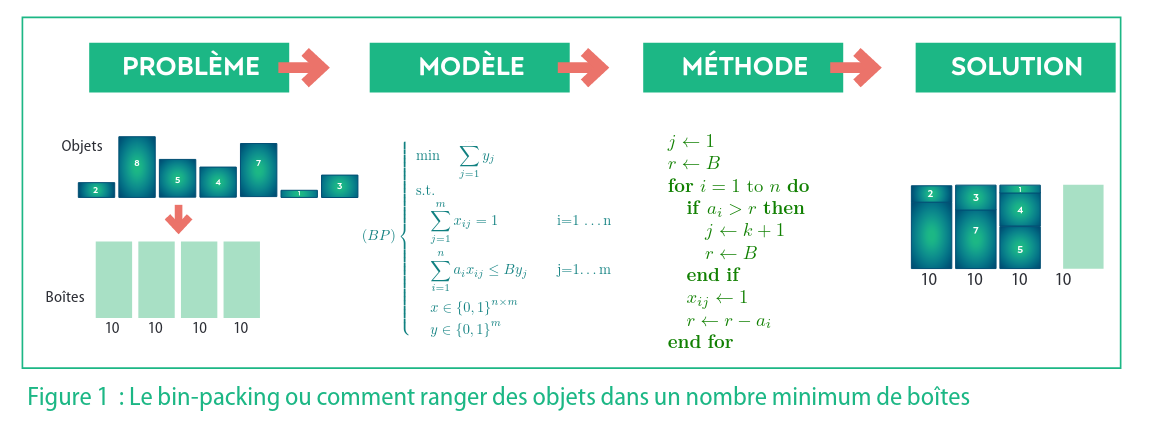
\includegraphics{img/bin-packing.png}
    }
\end{figure}
\end{document}
